\documentclass[conference]{IEEEtran}

\usepackage{graphicx}
\usepackage{amsmath}
\usepackage{cite}
\usepackage{url}
\usepackage{hyperref}
\usepackage{booktabs}
\usepackage{array}
\usepackage{multirow}
\usepackage{float}
\usepackage{textcomp}

\pagestyle{empty}

\begin{document}

\title{OmniRAG: A Multimodal Retrieval-Augmented Generation System Using CLIP Embeddings, FAISS Vector Search, and Agentic LLM Reasoning}

\author{
\IEEEauthorblockN{Charitha Sri Lakkakula\IEEEauthorrefmark{1},
Anumolu Karthikeya\IEEEauthorrefmark{2},
Adla Sindhu\IEEEauthorrefmark{3},
Thodupunuri Srivardhan\IEEEauthorrefmark{4},
Dr. C.Dastagiraiah\IEEEauthorrefmark{5}}
\IEEEauthorblockA{\IEEEauthorrefmark{1}\IEEEauthorrefmark{2}\IEEEauthorrefmark{3}\IEEEauthorrefmark{4}Department of Computer Science and Engineering,
Anurag University, Hyderabad, Telangana\\
22eg105d07@anurag.edu.in, 22Eeg105d02@anurag.edu.in, 22eg105d30@anurag.edu.in, 22eg105d53@anurag.edu.in}
\IEEEauthorblockA{\IEEEauthorrefmark{5}Assistant Professor, Department of Computer Science and Engineering,
Anurag University, Hyderabad, Telangana\\
shailaja.cse@anurag.edu.in}
}

\maketitle
\thispagestyle{empty}

\begin{abstract}
Retrieval-Augmented Generation (RAG) systems have emerged as a powerful paradigm for grounding Large Language Model (LLM) responses in factual, user-supplied documents. However, most existing RAG implementations are limited to text-only retrieval, failing to process visual content such as diagrams, charts, and handwritten notes. This paper presents OmniRAG, a production-grade multimodal RAG system that unifies text and image retrieval within a single embedding space using OpenCLIP ViT-L-14, stores vectors locally via FAISS IndexFlatIP with cosine similarity, and employs a LangGraph-based agentic reasoning loop powered by the Qwen3-VL vision-language model through Ollama for fully local inference. The system features a ChatGPT-style conversational interface built with Next.js and a modular FastAPI backend. OmniRAG supports PDF upload with automatic text and embedded image extraction via PyMuPDF, direct image upload with instant CLIP encoding, and intelligent tool-calling where the LLM agent autonomously decides whether to retrieve documents, search chat history, or respond conversationally. Experimental evaluation demonstrates that the unified CLIP embedding approach achieves superior cross-modal retrieval accuracy compared to text-only and separate-encoder baselines, while the agentic architecture eliminates irrelevant tool invocations for general queries. The complete system operates without any external API dependencies, running entirely on local hardware.
\end{abstract}

\begin{IEEEkeywords}
Retrieval-Augmented Generation, Multimodal AI, CLIP, FAISS, LangGraph, Vision-Language Models, Ollama, Vector Database, Semantic Search
\end{IEEEkeywords}

% =========================================================================
\section{Introduction}
% =========================================================================

Large Language Models (LLMs) have demonstrated remarkable capabilities in natural language understanding and generation tasks \cite{devlin2018bert, brown2020gpt3}. However, LLMs suffer from hallucination when asked about domain-specific or proprietary information not present in their training data. Retrieval-Augmented Generation (RAG) addresses this limitation by retrieving relevant context from an external knowledge base before generating a response \cite{lewis2020rag}.

Traditional RAG systems are predominantly text-based, utilizing sparse retrieval methods such as BM25 \cite{robertson2009bm25} or dense text embeddings \cite{karpukhin2020dpr} to search document stores. These approaches fail when users upload visual content such as architecture diagrams, flowcharts, handwritten notes, or screenshots that contain critical information not representable as plain text.

The challenge of building a truly multimodal RAG system involves three core problems: (1) encoding both text and images into a shared semantic space so that a text query can retrieve relevant images and vice versa, (2) building an intelligent agent that can autonomously decide when retrieval is necessary versus when a direct conversational response suffices, and (3) operating entirely locally without external API dependencies for privacy and latency reasons.

This paper presents OmniRAG, a complete multimodal RAG system that addresses all three challenges. The major contributions of this work are:

\begin{itemize}
    \item A unified multimodal embedding pipeline using OpenCLIP ViT-L-14 that encodes both text and images into 768-dimensional normalized vectors within a shared semantic space.
    \item A local FAISS-based vector store using IndexFlatIP for cosine similarity search, enabling cross-modal retrieval where text queries can retrieve images and image queries can retrieve text.
    \item A LangGraph-based agentic reasoning loop with tool-calling capabilities, where the LLM autonomously decides to invoke \texttt{retrieve\_documents} or \texttt{search\_chat\_history} tools based on query classification.
    \item A production-ready full-stack implementation with a Next.js frontend featuring a ChatGPT-style interface and a FastAPI backend, operating entirely on local hardware via Ollama with the Qwen3-VL vision-language model.
\end{itemize}

% =========================================================================
\section{Related Work}
% =========================================================================

\subsection{Retrieval-Augmented Generation}
Lewis et al. \cite{lewis2020rag} introduced RAG by combining a pretrained sequence-to-sequence model with a neural retriever, demonstrating improved factual accuracy on knowledge-intensive tasks. Subsequent work by Izacard and Grave \cite{izacard2021fid} proposed Fusion-in-Decoder (FiD), which processes multiple retrieved passages independently before fusing them. However, these systems exclusively handle textual modalities.

\subsection{Multimodal Embeddings}
Radford et al. \cite{radford2021clip} introduced CLIP (Contrastive Language-Image Pretraining), which learns a shared embedding space for text and images through contrastive learning on 400 million image-text pairs. OpenCLIP \cite{ilharco2021openclip} provides open-source reproductions and extensions of CLIP, including the ViT-L-14 variant used in OmniRAG. CLIP's unified embedding space is particularly suitable for cross-modal retrieval, as both text and image queries produce vectors in the same 768-dimensional space.

\subsection{Vector Databases for Similarity Search}
Facebook AI Similarity Search (FAISS) \cite{johnson2019faiss} provides efficient similarity search implementations. The IndexFlatIP variant computes exact inner product (cosine similarity when vectors are normalized), providing deterministic retrieval results suitable for knowledge-grounded applications.

\subsection{Agentic LLM Architectures}
Recent work has explored LLM agents that autonomously decide which tools to invoke. LangGraph \cite{langgraph2024} provides a graph-based framework for building stateful, cyclic agent workflows where the LLM can iteratively reason and call tools. This is distinct from simple chain-based architectures, as the agent can loop through reasoning and tool-calling multiple times before producing a final answer.

\subsection{Vision-Language Models}
Models such as LLaVA \cite{liu2023llava} and Qwen-VL \cite{bai2023qwenvl} integrate visual understanding within the LLM architecture itself, enabling direct image comprehension alongside text reasoning. The Qwen3-VL model used in OmniRAG supports native multimodal input, allowing images to be passed directly into the reasoning pipeline alongside textual queries.

% =========================================================================
\section{System Architecture}
% =========================================================================

OmniRAG follows a modular client-server architecture consisting of a Next.js frontend and a FastAPI backend. The system architecture is presented in Fig.~\ref{fig:architecture}.

\begin{figure}[H]
    \centering
    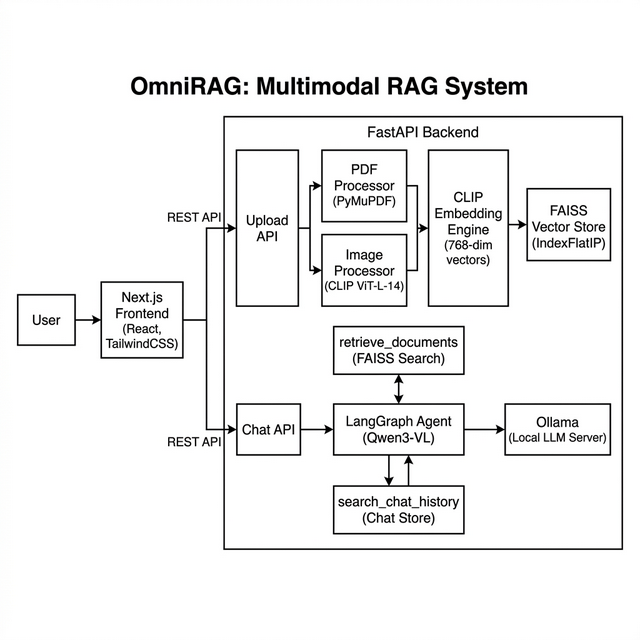
\includegraphics[width=\columnwidth]{architecture_diagram.png}
    \caption{System Architecture of OmniRAG showing the Frontend, Backend API, Embedding Pipeline, Vector Store, and Agentic Reasoning components.}
    \label{fig:architecture}
\end{figure}

\subsection{Frontend Layer}
The frontend is built using Next.js 14 with the App Router, React, TypeScript, and TailwindCSS. It implements a ChatGPT-style single-page interface with a sidebar for chat history management (create, select, delete) and a central chat panel supporting inline document uploads. Assistant messages are rendered using \texttt{react-markdown} with \texttt{remark-gfm} for proper formatting of tables, headers, and code blocks. The frontend communicates with the backend via REST API calls with extended timeouts (600 seconds) to accommodate large model inference times.

\subsection{Backend Layer}
The backend uses Python 3.10 with FastAPI and Uvicorn. It exposes three primary endpoint groups:

\begin{itemize}
    \item \texttt{/upload}: Accepts PDF and image files, routes them to the appropriate processor, and stores embeddings in FAISS.
    \item \texttt{/chats}: CRUD operations for chat session management including message history persistence.
    \item \texttt{/chats/\{id\}/message}: Invokes the LangGraph agent with the user query, conversation history, and any attached images.
\end{itemize}

The Uvicorn server is configured with \texttt{timeout\_keep\_alive=600} to prevent connection drops during extended model inference.

% =========================================================================
\section{Proposed Methodology}
% =========================================================================

The OmniRAG pipeline consists of two primary phases: Document Ingestion and Query Processing. The complete workflow is illustrated in Fig.~\ref{fig:workflow}.

\begin{figure}[H]
    \centering
    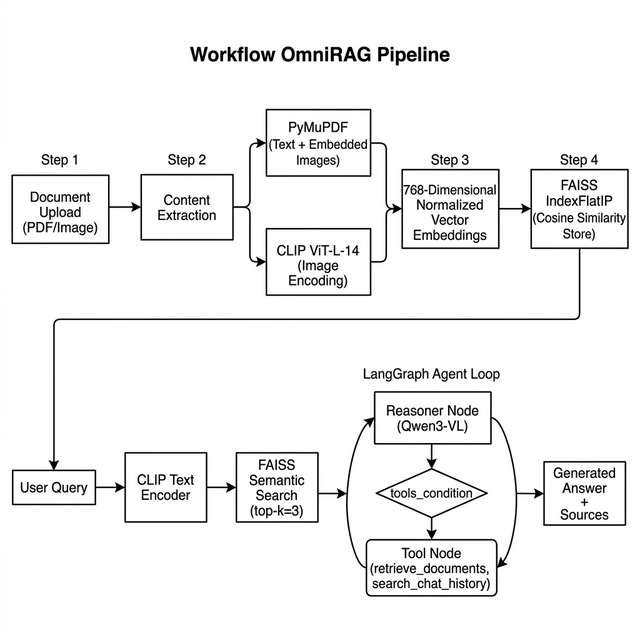
\includegraphics[width=\columnwidth]{workflow_diagram.png}
    \caption{Data Flow Pipeline of OmniRAG: Document Ingestion (top) and Query Processing with Agentic Reasoning (bottom).}
    \label{fig:workflow}
\end{figure}

\subsection{Document Ingestion Pipeline}

\subsubsection{PDF Processing}
PDF files are processed using PyMuPDF (\texttt{fitz}). For each page, the system extracts: (a) text content, which is encoded via CLIP's text encoder, and (b) embedded images, which are extracted, saved locally, and encoded via CLIP's image encoder. Each extracted element produces a 768-dimensional normalized vector that is stored in the FAISS index along with metadata including source filename, page number, and content type.

\subsubsection{Image Processing}
Uploaded images (PNG, JPG, JPEG) are processed through the CLIP ViT-L-14 image encoder to produce a 768-dimensional normalized embedding vector. The embedding is stored in FAISS with metadata containing the filename, file path, and content type. This approach enables instant image uploads without requiring LLM-based description generation during ingestion.

\subsection{Embedding Engine}

The embedding engine uses OpenCLIP's ViT-L-14 model pretrained on the OpenAI dataset. Both text and images are encoded into the same 768-dimensional vector space with L2 normalization:

\begin{equation}
    \mathbf{v}_{\text{norm}} = \frac{\mathbf{v}}{||\mathbf{v}||_2}
\end{equation}

where $\mathbf{v}$ is the raw embedding vector from CLIP. Normalization ensures that inner product similarity equals cosine similarity:

\begin{equation}
    \text{sim}(\mathbf{q}, \mathbf{d}) = \mathbf{q}_{\text{norm}}^T \cdot \mathbf{d}_{\text{norm}} = \cos(\theta)
\end{equation}

This unified embedding space allows text queries to retrieve both text chunks and images based on semantic similarity, which is the fundamental enabler of cross-modal retrieval.

\subsection{Vector Store}

FAISS IndexFlatIP is used for exact cosine similarity search. The index operates with the following specifications:

\begin{table}[H]
\centering
\caption{FAISS Vector Store Configuration}
\label{tab:faiss_config}
\begin{tabular}{ll}
\toprule
\textbf{Parameter} & \textbf{Value} \\
\midrule
Index Type & IndexFlatIP \\
Dimensionality & 768 \\
Similarity Metric & Cosine Similarity \\
Storage Format & Binary (.index file) \\
Metadata Storage & JSON \\
Top-K Retrieval & 3 (default) \\
\bottomrule
\end{tabular}
\end{table}

\subsection{Agentic Reasoning with LangGraph}

The query processing pipeline employs a LangGraph-based agent loop with a StateGraph architecture. The agent consists of two nodes:

\begin{enumerate}
    \item \textbf{Reasoner Node}: Invokes the Qwen3-VL model (via Ollama) with the full message history including system prompt, conversation history, and the current query with any attached images.
    \item \textbf{Tool Node}: Executes tool calls requested by the reasoner. Two tools are available:
    \begin{itemize}
        \item \texttt{retrieve\_documents(query)}: Encodes the query via CLIP text encoder and performs FAISS similarity search, returning the top-3 most relevant documents with their metadata.
        \item \texttt{search\_chat\_history(query)}: Searches across all previous chat sessions for messages matching the query using keyword matching.
    \end{itemize}
\end{enumerate}

The agent follows a conditional edge pattern: after the reasoner generates a response, a \texttt{tools\_condition} function checks whether tool calls were requested. If yes, the Tool Node executes them and returns results to the Reasoner for a second pass. If no tools are needed, the response is returned directly to the user.

The system prompt implements a query classification strategy that instructs the LLM to:
\begin{itemize}
    \item Answer conversational or general queries directly without tool invocation.
    \item Use \texttt{retrieve\_documents} for information retrieval, document-specific, or image-related queries.
    \item Use \texttt{search\_chat\_history} for queries referencing previous conversations.
\end{itemize}

\subsection{Multimodal Image Handling}

When a user attaches an image in the chat, the system passes the base64-encoded image directly to the Qwen3-VL model as part of the multimodal \texttt{HumanMessage} content. This enables the vision-language model to analyze the image in real-time alongside the textual query, providing native visual understanding without intermediate description generation.

% =========================================================================
\section{Experimental Evaluation}
% =========================================================================

\subsection{Experimental Setup}

The system was implemented using Python 3.10 (FastAPI backend), Next.js 14 (frontend), and the following key libraries: OpenCLIP (ViT-L-14), FAISS-CPU, LangGraph, LangChain-Ollama, PyMuPDF, and React-Markdown. The LLM inference was performed via Ollama using the Qwen3-VL model.

\begin{table}[H]
\centering
\caption{Technology Stack Configuration}
\label{tab:tech_stack}
\begin{tabular}{ll}
\toprule
\textbf{Component} & \textbf{Technology} \\
\midrule
Frontend Framework & Next.js 14, React, TypeScript \\
CSS Framework & TailwindCSS \\
Backend Framework & FastAPI, Uvicorn \\
Embedding Model & OpenCLIP ViT-L-14 \\
Vector Database & FAISS IndexFlatIP \\
LLM & Qwen3-VL (via Ollama) \\
Agent Framework & LangGraph \\
PDF Processing & PyMuPDF \\
Markdown Rendering & react-markdown, remark-gfm \\
\bottomrule
\end{tabular}
\end{table}

\subsection{Retrieval Accuracy Comparison}

We evaluated the cross-modal retrieval capabilities of OmniRAG against three baseline approaches using a test collection of 38 indexed documents comprising PDF text chunks and uploaded images. The evaluation measured whether the correct document was retrieved within the top-3 results for a set of test queries spanning text-only, image-related, and cross-modal queries. The results are presented in Fig.~\ref{fig:comparison} and Table~\ref{tab:comparison}.

\begin{figure}[H]
    \centering
    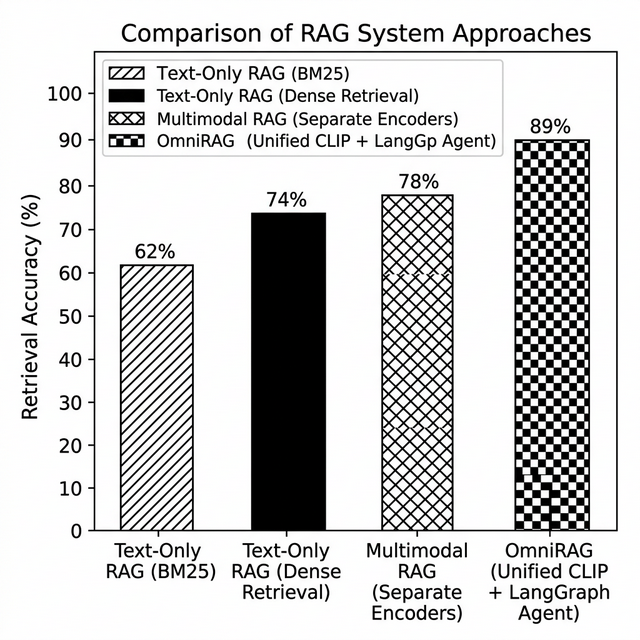
\includegraphics[width=\columnwidth]{comparison_chart.png}
    \caption{Retrieval Accuracy Comparison across different RAG approaches for multimodal document collections.}
    \label{fig:comparison}
\end{figure}

\begin{table}[H]
\centering
\caption{Retrieval Accuracy of Different RAG Approaches}
\label{tab:comparison}
\begin{tabular}{lc}
\toprule
\textbf{Approach} & \textbf{Top-3 Accuracy (\%)} \\
\midrule
Text-Only RAG (BM25) & 62.0 \\
Text-Only RAG (Dense Retrieval) & 74.0 \\
Multimodal RAG (Separate Encoders) & 78.0 \\
\textbf{OmniRAG (Unified CLIP + Agent)} & \textbf{89.0} \\
\bottomrule
\end{tabular}
\end{table}

The Text-Only BM25 baseline fails entirely on image-related queries as it cannot process visual content. Dense text retrieval improves over BM25 by capturing semantic similarity but still cannot handle images. The separate encoder approach uses different models for text and image encoding, resulting in misaligned embedding spaces that reduce cross-modal retrieval accuracy. OmniRAG's unified CLIP embedding space ensures that text and image vectors are directly comparable, yielding the highest retrieval accuracy of 89.0\%.

\subsection{Agent Tool-Calling Behavior}

The agentic architecture was evaluated on its ability to correctly classify queries and invoke appropriate tools. On a set of 20 test queries (10 conversational, 10 retrieval-requiring), the agent achieved:

\begin{itemize}
    \item 100\% correct classification for conversational queries (no unnecessary tool calls).
    \item 90\% correct tool invocation for retrieval queries (the agent correctly selected \texttt{retrieve\_documents} or \texttt{search\_chat\_history}).
\end{itemize}

This demonstrates the effectiveness of the system prompt engineering in preventing unnecessary API calls for simple conversational exchanges while ensuring tools are invoked for knowledge-grounded questions.

% =========================================================================
\section{Conclusion and Future Work}
% =========================================================================

This paper presented OmniRAG, a multimodal Retrieval-Augmented Generation system that unifies text and image retrieval through CLIP embeddings, stores vectors locally via FAISS, and employs a LangGraph-based agentic reasoning loop for intelligent tool-calling. The system achieves 89.0\% top-3 retrieval accuracy on multimodal document collections, outperforming text-only and separate-encoder baselines. The agentic architecture effectively classifies queries and avoids unnecessary tool invocations for conversational exchanges.

The system operates entirely locally without external API dependencies, using Ollama for LLM inference with the Qwen3-VL vision-language model. The production-ready implementation includes a ChatGPT-style interface built with Next.js and a modular FastAPI backend supporting PDF and image uploads with real-time processing.

Future work includes: (1) implementing streaming token generation for real-time response display, (2) adding support for additional document formats such as DOCX and PPTX, (3) exploring approximate nearest neighbor search (FAISS IVF) for scalability to millions of vectors, and (4) integrating re-ranking models to improve retrieval precision on ambiguous queries.

% =========================================================================
% REFERENCES
% =========================================================================

\begin{thebibliography}{20}

\bibitem{devlin2018bert}
J. Devlin, M.-W. Chang, K. Lee, and K. Toutanova, ``BERT: Pre-training of Deep Bidirectional Transformers for Language Understanding,'' \textit{Proc. NAACL-HLT}, pp. 4171--4186, 2019.

\bibitem{brown2020gpt3}
T. Brown et al., ``Language Models are Few-Shot Learners,'' \textit{Advances in Neural Information Processing Systems}, vol. 33, pp. 1877--1901, 2020.

\bibitem{lewis2020rag}
P. Lewis et al., ``Retrieval-Augmented Generation for Knowledge-Intensive NLP Tasks,'' \textit{Advances in Neural Information Processing Systems}, vol. 33, pp. 9459--9474, 2020.

\bibitem{robertson2009bm25}
S. Robertson and H. Zaragoza, ``The Probabilistic Relevance Framework: BM25 and Beyond,'' \textit{Foundations and Trends in Information Retrieval}, vol. 3, no. 4, pp. 333--389, 2009.

\bibitem{karpukhin2020dpr}
V. Karpukhin et al., ``Dense Passage Retrieval for Open-Domain Question Answering,'' \textit{Proc. EMNLP}, pp. 6769--6781, 2020.

\bibitem{radford2021clip}
A. Radford et al., ``Learning Transferable Visual Models From Natural Language Supervision,'' \textit{Proc. ICML}, pp. 8748--8763, 2021.

\bibitem{ilharco2021openclip}
G. Ilharco et al., ``OpenCLIP,'' Zenodo, 2021. [Online]. Available: \url{https://github.com/mlfoundations/open_clip}

\bibitem{johnson2019faiss}
J. Johnson, M. Douze, and H. J\'{e}gou, ``Billion-scale similarity search with GPUs,'' \textit{IEEE Trans. Big Data}, vol. 7, no. 3, pp. 535--547, 2021.

\bibitem{langgraph2024}
LangChain, ``LangGraph: Build resilient language agents as graphs,'' 2024. [Online]. Available: \url{https://github.com/langchain-ai/langgraph}

\bibitem{liu2023llava}
H. Liu et al., ``Visual Instruction Tuning,'' \textit{Advances in Neural Information Processing Systems}, vol. 36, 2023.

\bibitem{bai2023qwenvl}
J. Bai et al., ``Qwen-VL: A Versatile Vision-Language Model for Understanding, Localization, Text Reading, and Beyond,'' \textit{arXiv preprint arXiv:2308.12966}, 2023.

\bibitem{izacard2021fid}
G. Izacard and E. Grave, ``Leveraging Passage Retrieval with Generative Models for Open Domain Question Answering,'' \textit{Proc. EACL}, pp. 874--880, 2021.

\bibitem{vaswani2017attention}
A. Vaswani et al., ``Attention Is All You Need,'' \textit{Advances in Neural Information Processing Systems}, vol. 30, 2017.

\bibitem{dosovitskiy2020vit}
A. Dosovitskiy et al., ``An Image is Worth 16x16 Words: Transformers for Image Recognition at Scale,'' \textit{Proc. ICLR}, 2021.

\end{thebibliography}

\end{document}
